
\renewcommand{\EntradaBibtex}{ConteoSentadillas_UPV_2024}

\begin{frame}{\citetitle{\EntradaBibtex}$^*$ (1)}
\begin{block}{Motivación} 
Se requiere una herramienta para verificar que las personas hagan los ejercicios de manera correcta
\begin{itemize}
\item Se implementó una aplicación móvil
\begin{itemize}
\item Permite al usuario llevar el conteo de sentadillas, tanto se las hace de frente como de lado.
\item Debe ubicar el dispositivo a una distancia de 80 cm. 
\item Si el ejercicio no es bien realizado, no se contabiliza.
\end{itemize}
\end{itemize}
\end{block} 
\begin{center}
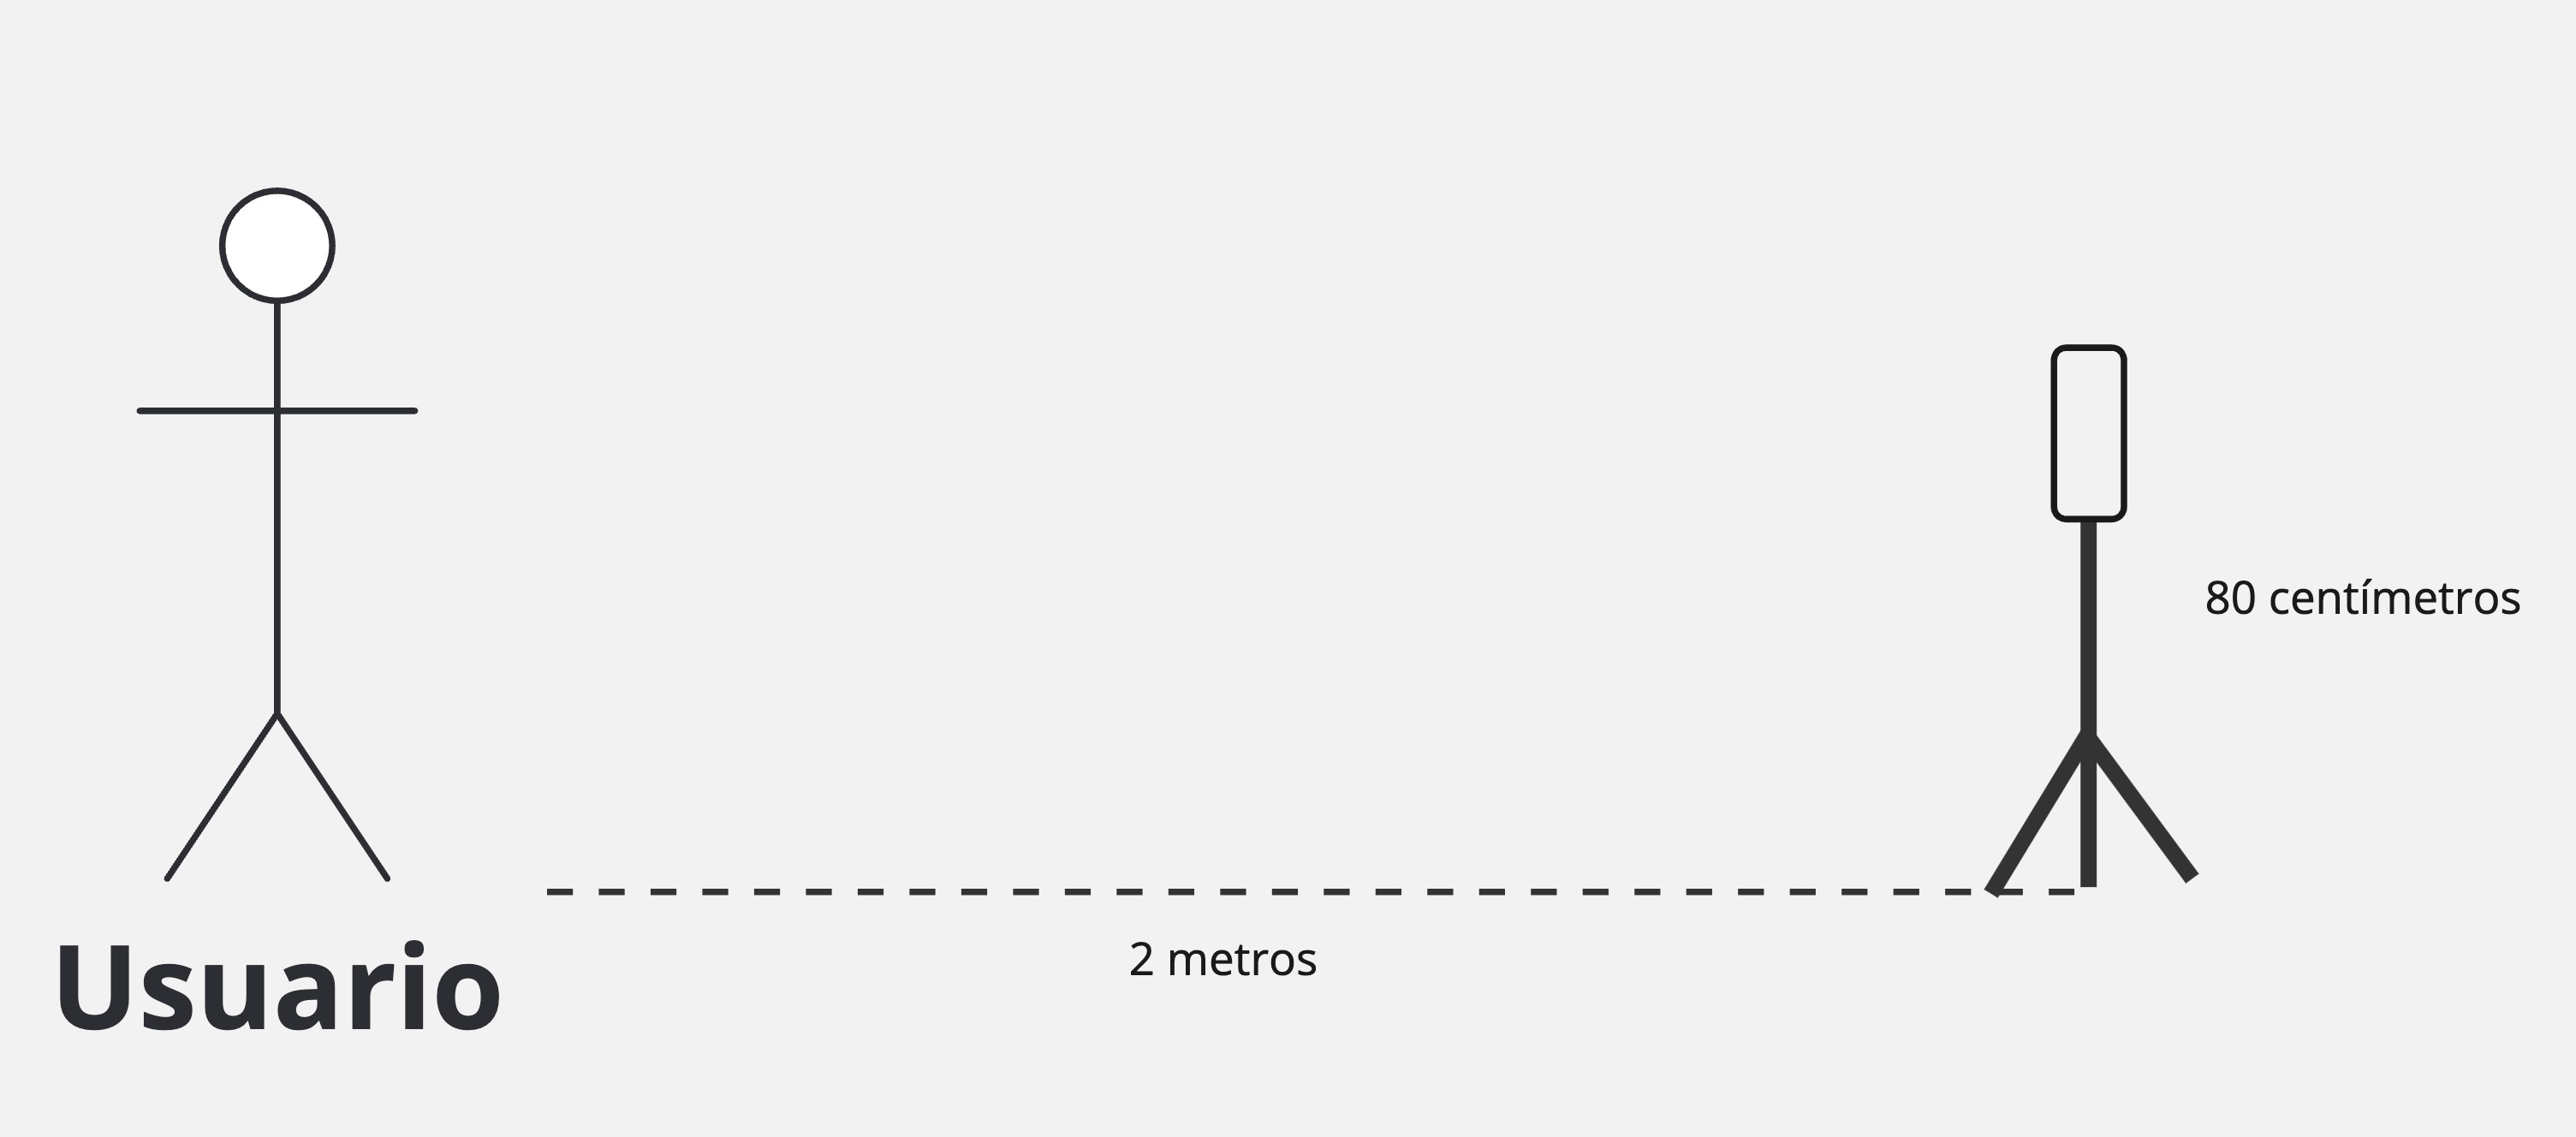
\includegraphics[width=0.48\linewidth]{2024_ConteoSentadillas/Ilustrativa.jpg}
\end{center}
\footfullcite*{\EntradaBibtex}
\end{frame}


\begin{frame}{\citetitle{\EntradaBibtex} (2)}
%\begin{block}{Pantallas Principales} 

\begin{columns}
% Column 1
\column{.5\linewidth}



\begin{center}
	\begin{tabular}{cc}
		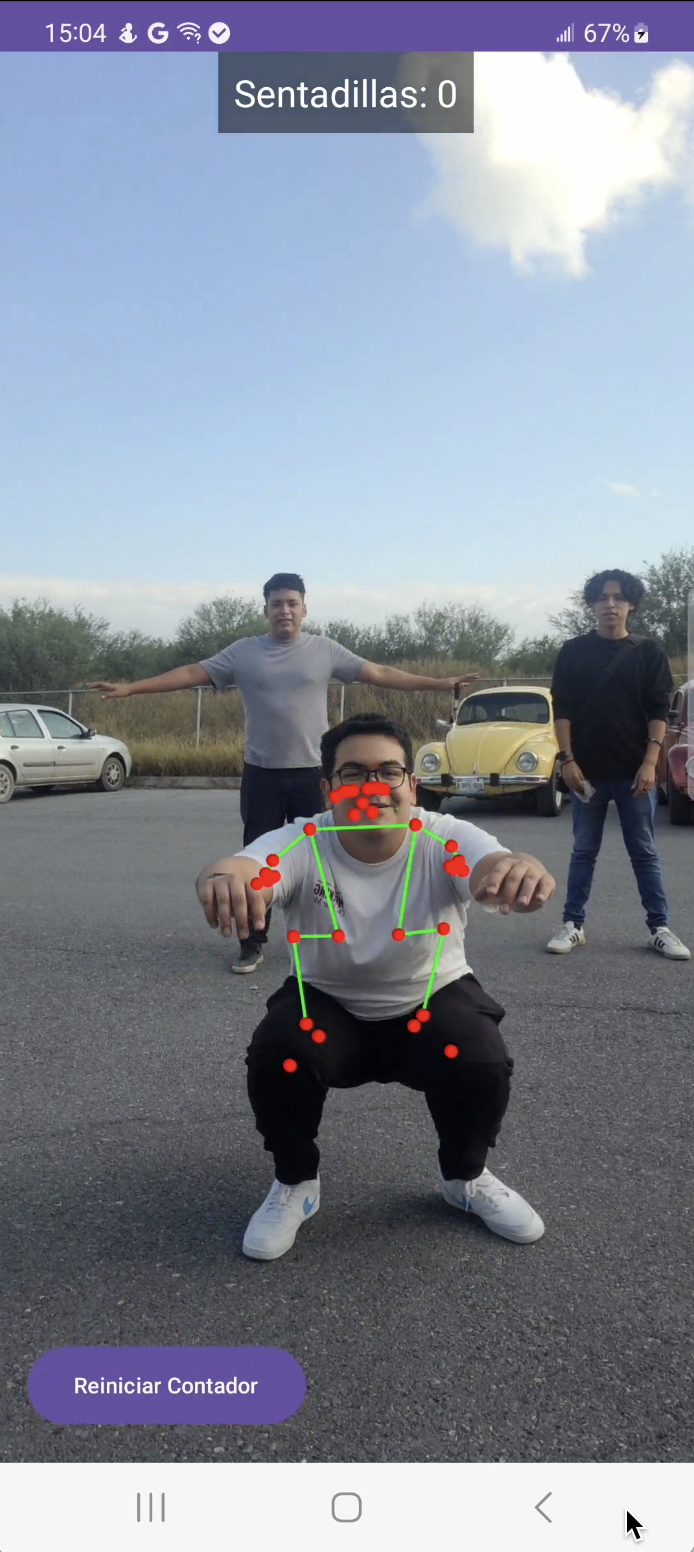
\includegraphics[width=0.40\linewidth]{2024_ConteoSentadillas/comienzo-sentadilla.png} &
		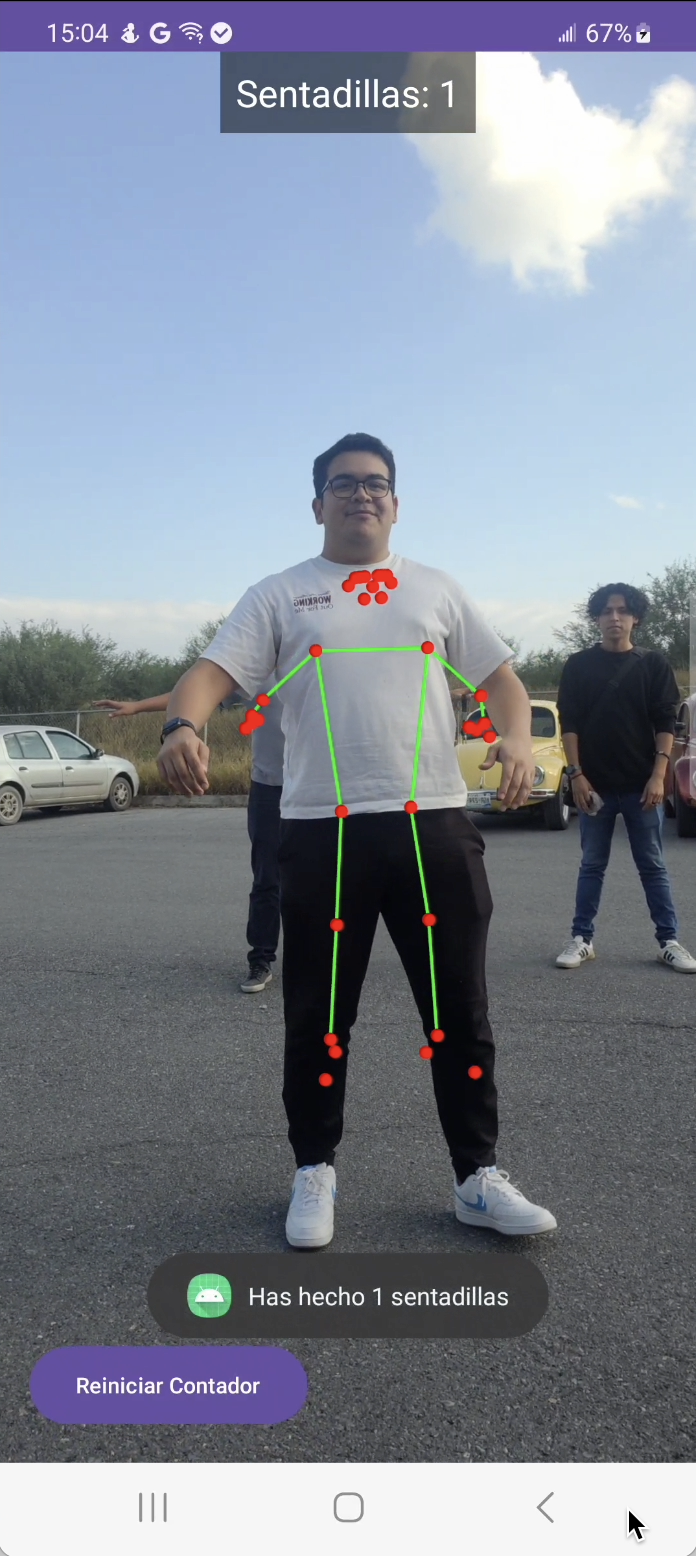
\includegraphics[width=0.40\linewidth]{2024_ConteoSentadillas/fin-sentadilla.png} \\
	\end{tabular}
\end{center}

\column{.5\linewidth}
\begin{center}
	\begin{tabular}{cccc}
		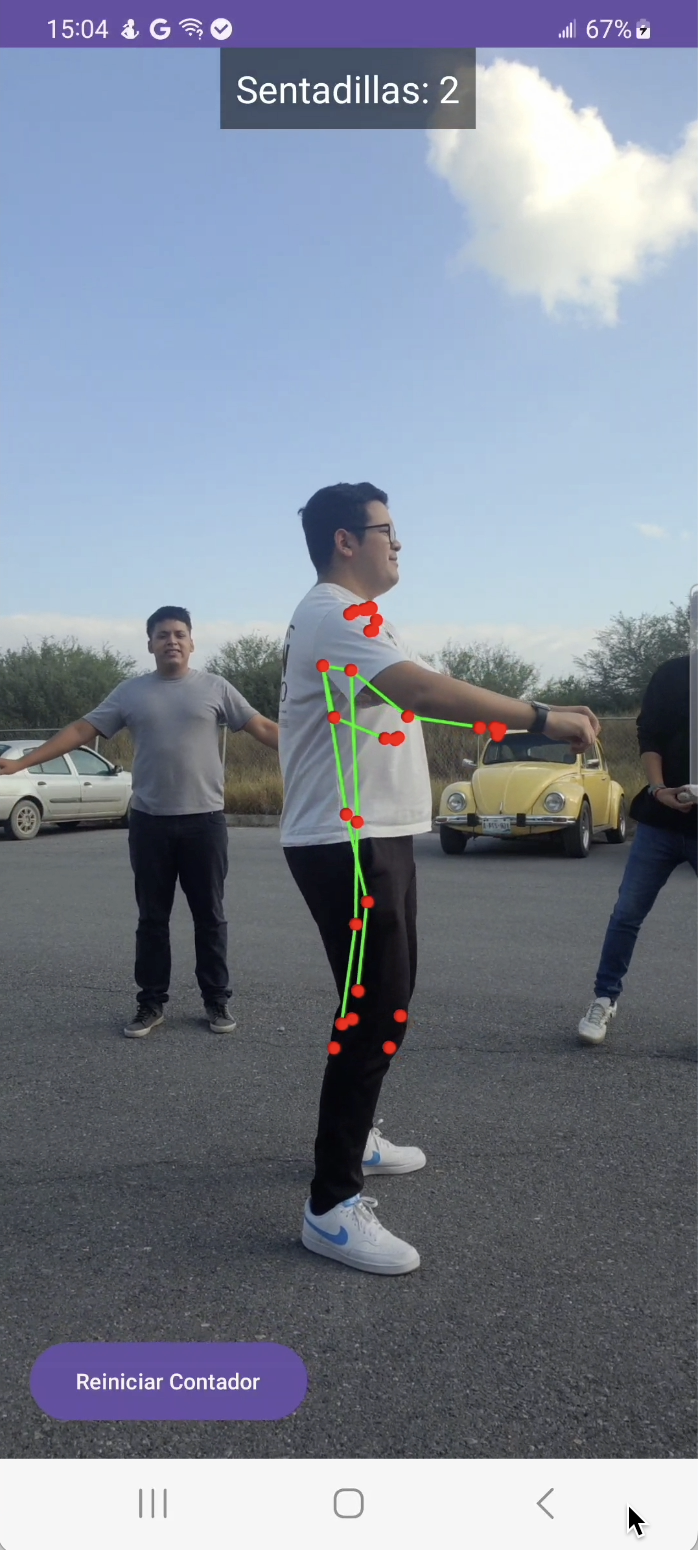
\includegraphics[width=0.40\linewidth]{2024_ConteoSentadillas/sentadilla-lateral-inicio.png} &
 		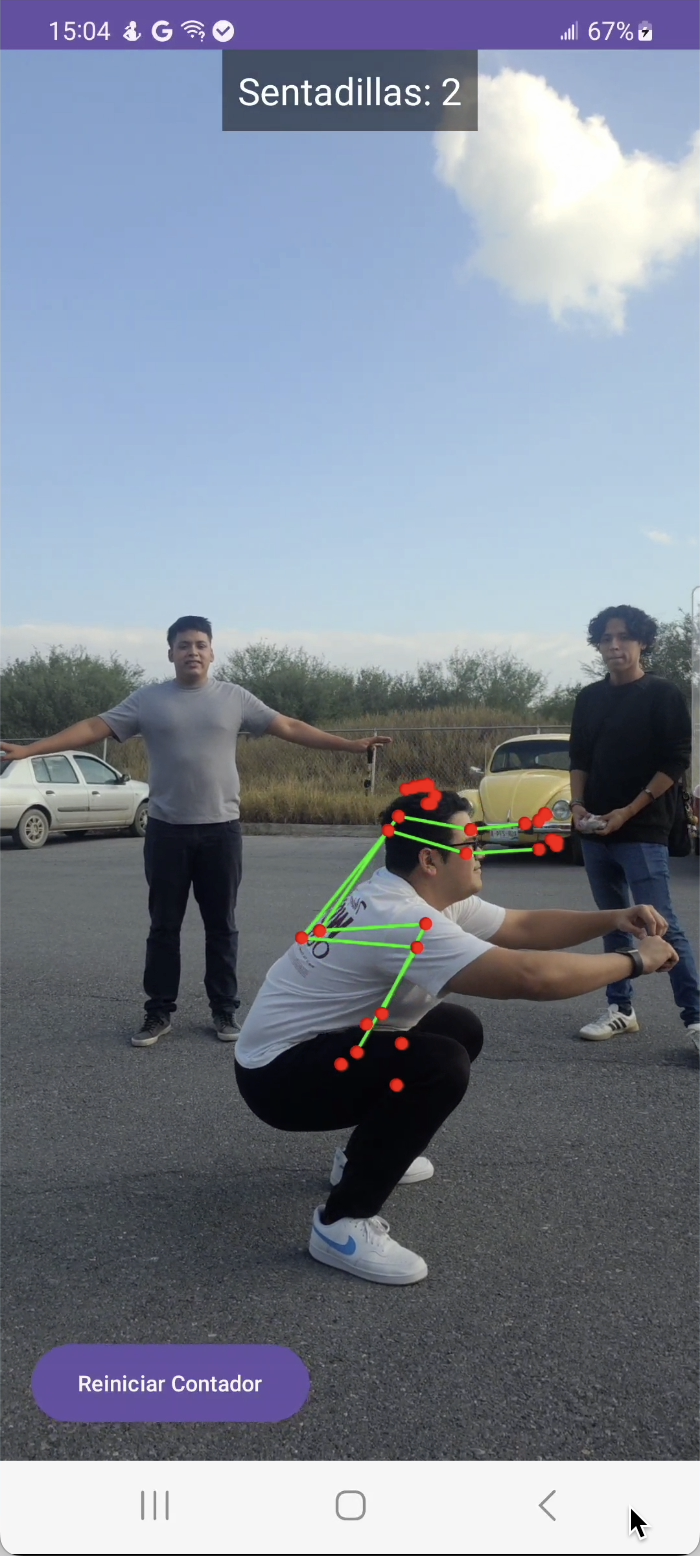
\includegraphics[width=0.40\linewidth]{2024_ConteoSentadillas/sentadilla-lateral-proceso.png} \\
	\end{tabular}
\end{center}


\end{columns}
\end{frame}


